

 \subsubsection{Senkrechte Polarisation}
% 
\begin{tikzpicture}
    \draw[dotted] (-3,0) -- (3,0);
    \draw[-] (0,-4) -- (0,4)                node[below right] {$\varepsilon_{r2}, \mu_{r2}, \sigma_{r2}$}
                                            node[below left] {$\varepsilon_{r1}, \mu_{r1}, \sigma_{r1}$};

    \draw[->] (-3,3) -- (-1.5,1.5)          node[above right] {$S_h$};
    \draw[->] (-3,3) -- (-3.5,2.5)          node[below right] {$H_h$};
    \draw[-] (-3,3) circle (0.15)           node[above] {$E_h$};
    \draw[dotted] (-3,3) -- (0,0);
    \draw[<->] (135:0.5) arc (135:180:0.5); 
    \node[] at (-0.8,0.2) {$\alpha$};

    \draw[->] (-1.5,-1.5) -- (-2,-2)        node[above left] {$S_r$};
    \draw[->] (-1.5,-1.5) -- (-1.8,-1.2)    node[above] {$H_r$};
    \draw[-] (-1.5,-1.5) circle (0.15)      node[right] {$E_r$};
    \draw[dotted] (-3,-3) -- (0,0);
    \draw[<->] (180:0.5) arc (180:225:0.5);
    \node[] at (-0.8,-0.2) {$\alpha$};

    \draw[->] (2,-0.6666) -- (3,-1)         node[above right] {$S_g$};
    \draw[->] (2,-0.6666) -- (1.3333,-2.8)  node[below right] {$H_g$};
    \draw[-] (2,-0.6666) circle (0.15)      node[above] {$E_g$};
    \draw[dotted] (0,0) -- (3,-1);
    \draw[<->] (0:1) arc (0:-20:1);     
    \node[] at (1.3,-0.2) {$\beta$};

\end{tikzpicture}
%  \subsection{Kopie}
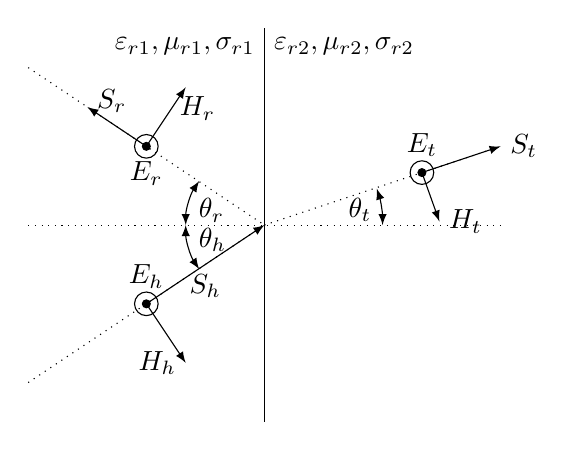
\begin{tikzpicture}
    \tikzset{cross/.style={cross out, draw=black, minimum size=2*(#1-\pgflinewidth), inner sep=0pt, outer sep=0pt},
        %     %default radius will be 1pt. 
        cross/.default={3.5pt}}
    %Kreuz
    \draw[dotted] (-3,0) -- (3,0);
    \draw[-] (0,-2.5) -- (0,2.5)                
        node[below right]   {$\varepsilon_{r2}, \mu_{r2}, \sigma_{r2}$}
        node[below left]    {$\varepsilon_{r1}, \mu_{r1}, \sigma_{r1}$};
    %Rücklaufende
    \draw[-latex] (-1.5,1) -- (-2.25,1.5)   node[right, yshift=.5ex]{$S_r$};
    \draw[-latex] (-1.5,1) -- (-1,1.75)     node[below, xshift=1ex] {$H_r$};
    \draw[-] (-1.5,1) circle (0.15)         node[below,yshift=-.5ex]{$E_r$};
    \draw[-,fill=black!100] (-1.5,1) circle (0.05);
    \draw[dotted] (-3,2) -- (0,0);
    \draw[latex-latex] (146:1) arc (146:180:1) 
        node[midway, right, yshift=-.7ex] {$\theta_r$};

    %Hinlaufende
    \draw[-latex] (-1.5,-1) -- (0,0)        node[below, midway]         {$S_h$};
    \draw[-latex] (-1.5,-1) -- (-1,-1.75)   node[left]                  {$H_h$};
    \draw[-] (-1.5,-1) circle (0.15)        node[above, yshift=.5ex]    {$E_h$};
    \draw[-,fill=black!100] (-1.5,-1) circle (0.05);
    \draw[dotted] (-3,-2) -- (0,0);
    \draw[latex-latex] (180:1) arc (180:214:1)
        node[midway, right, yshift=.7ex] {$\theta_h$};

    %Transmitierte
    \draw[-latex] (2,0.6666) -- (3,1)           node[right] {$S_t$};
    \draw[-latex] (2,0.6666) -- (2.2223,0.0448) node[right] {$H_t$};
    \draw[-] (2,0.6666) circle (0.15)           node[above, yshift=.5ex] {$E_t$};
    \draw[-,fill=black!100] (2,0.6666) circle (0.05);
    \draw[dotted] (0,0) -- (3,1);
    \draw[latex-latex] (0:1.5) arc (0:18:1.5)
        node[midway, left, yshift=-.3ex] {$\theta_t$};

\end{tikzpicture}

\begin{itemize}
    \item mag./elek. Reflexionsfaktor $[1]$
    \item mag. Transmissionsfaktor $[1]$
    \item elek. Transmissionsfaktor $[1]$
\end{itemize}

\begin{align*}
    Z_{Fn}                            & = Z_{F0}\cdot\frac{1}{\sqrt{\varepsilon_{rn}}}                                                                                                                  \\
    \frac{Z_{F1}}{Z_{F2}}             & = \frac{\sqrt{\varepsilon_{r2}}}{\sqrt{\varepsilon_{r1}}}                                                                                                       \\
    \frac{\sin\theta_t}{\sin\theta_h} & = \frac{\lambda_2}{\lambda_1}= \frac{\beta_1}{\beta_2}= \frac{n_1}{n_2} \qquad n: Brechungsindex                                                                \\
    \theta_h                          & = \theta_r                                                                                                                                                      \\
    \sin\theta_t                      & = \sqrt{\frac{\varepsilon_{r1}}{\varepsilon_{r2}}}\cdot\theta_h                                                                                                 \\
    r_s                               & =  r_{e s} = r_{m s} =                                                                                                                                          \\
                                      & = \frac{Z_{F 2} \cdot \cos \theta_h-Z_{F 1} \cdot \cos \theta_t}{Z_{F 2} \cdot \cos \theta_h+Z_{F 1} \cdot \cos \theta_t} =                                     \\
                                      & = \frac{\cos\theta_h-\sqrt{^{\varepsilon_{r2}}/_{\varepsilon_{r1}}-\sin^2\theta_h}}{\cos\theta_h+\sqrt{^{\varepsilon_{r2}}/_{\varepsilon_{r1}}-\sin^2\theta_h}} \\
    t_{m s}                           & = Z_{F 1} \cdot \frac{2 \cdot \cos \theta_h}{Z_{F 2} \cdot \cos \theta_h+Z_{F 1} \cdot \cos \theta_t}                                                           \\
                                      & = (1 - r_{s}) \cdot \dfrac{\cos \theta_h}{\cos \theta_t}                                                                                                        \\
                                      & = \frac{Z_{F1}}{Z_{F2}}\cdot t_{es}                                                                                                                             \\
    t_{e s}                           & = Z_{F 2} \cdot \frac{2 \cdot \cos \theta_h}{Z_{F 2} \cdot \cos \theta_h+Z_{F 1} \cdot \cos \theta_t}                                                           \\
                                      & = 1+r_{s}                                                                                                                                                       \\
    E_{r}                             & = r_{s} \cdot E_{h}                                                                                                                                             \\
    E_{t}                             & = t_{e s} \cdot E_{h}                                                                                                                                           \\
    H_{r}                             & = r_{s} \cdot H_{h}                                                                                                                                             \\
    H_{t}                             & = t_{m s} \cdot H_{h}
\end{align*}

\subsubsection{Parallel Polarisation}
% \begin{tikzpicture}
    \draw[dotted] (-3,0) -- (3,0);
    \draw[-] (0,-4) -- (0,4)                node[below right] {$\varepsilon_{r2}, \mu_{r2}, \sigma_{r2}$}
                                            node[below left] {$\varepsilon_{r1}, \mu_{r1}, \sigma_{r1}$};

    \draw[->] (-3,3) -- (-1.5,1.5)          node[above right] {$S_h$};
    \draw[->] (-3,3) -- (-3.5,2.5)          node[below right] {$E_h$};
    \draw[-] (-3,3) circle (0.15)           node[above] {$H_h$};
    \draw[dotted] (-3,3) -- (0,0);
    \draw[<->] (135:0.5) arc (135:180:0.5); 
    \node[] at (-0.8,0.2) {$\theta_h$};

    \draw[->] (-1.5,-1.5) -- (-2,-2)        node[above left] {$S_r$};
    \draw[->] (-1.5,-1.5) -- (-1.8,-1.2)    node[above] {$E_r$};
    \draw[-] (-1.5,-1.5) circle (0.15)      node[right] {$H_r$};
    \draw[dotted] (-3,-3) -- (0,0);
    \draw[<->] (180:0.5) arc (180:225:0.5);
    \node[] at (-0.8,-0.2) {$\theta_r$};

    \draw[->] (2,-0.6666) -- (3,-1)         node[above right] {$S_t$};
    \draw[->] (2,-0.6666) -- (1.3333,-2.8)  node[below right] {$E_t$};
    \draw[-] (2,-0.6666) circle (0.15)      node[above] {$H_t$};
    \draw[dotted] (0,0) -- (3,-1);
    \draw[<->] (0:1) arc (0:-20:1);     
    \node[] at (1.3,-0.2) {$\theta_t$};

\end{tikzpicture}
% \subsection{Kopie}
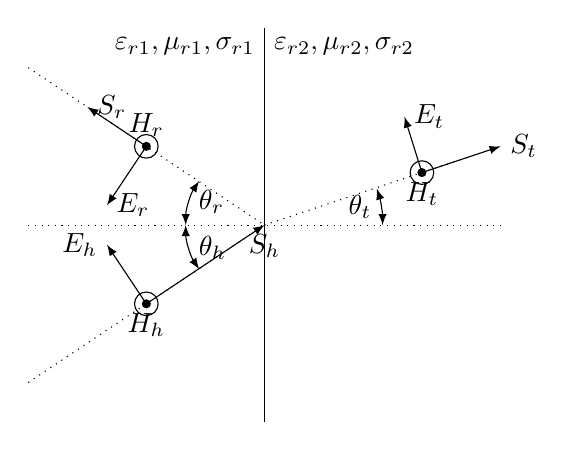
\begin{tikzpicture}
    \tikzset{cross/.style={cross out, draw=black, minimum size=2*(#1-\pgflinewidth), inner sep=0pt, outer sep=0pt},
        %     %default radius will be 1pt. 
        cross/.default={3.5pt}}
    %Kreunz
    \draw[dotted] (-3,0) -- (3,0);
    \draw[-] (0,-2.5) -- (0,2.5)                node[below right] {$\varepsilon_{r2}, \mu_{r2}, \sigma_{r2}$}
                                            node[below left] {$\varepsilon_{r1}, \mu_{r1}, \sigma_{r1}$};
    %Rücklaufende
    \draw[-latex] (-1.5,1) -- (-2.25,1.5)          node[right] {$S_r$};
    \draw[-latex] (-1.5,1) -- (-2,0.25)          node[right] {$E_r$};
    \draw[-] (-1.5,1) circle (0.15)           node[above] {$H_r$};
    \draw[-,fill=black!100] (-1.5,1) circle (0.05);
    \draw[dotted] (-3,2) -- (0,0);
    \draw[latex-latex] (146:1) arc (146:180:1) node[midway, right] {$\theta_r$};

    %Hinlaufende
    \draw[-latex] (-1.5,-1) -- (0,0)        node[below ] {$S_h$};
    \draw[-latex] (-1.5,-1) -- (-2,-0.25)    node[left] {$E_h$};
    \draw[-] (-1.5,-1) circle (0.15)      node[below] {$H_h$};
    \draw[-,fill=black!100] (-1.5,-1) circle (0.05);
    \draw[dotted] (-3,-2) -- (0,0);
    \draw[latex-latex] (180:1) arc (180:214:1) node[midway, right] {$\theta_h$};

    %Transmitierte
    \draw[-latex] (2,0.6666) -- (3,1)         node[right] {$S_t$};
    \draw[-latex] (2,0.6666) -- (1.7777,1.378)  node[right] {$E_t$};
    \draw[-] (2,0.6666) circle (0.15)      node[below] {$H_t$};
    \draw[-,fill=black!100] (2,0.6666) circle (0.05);
    \draw[dotted] (0,0) -- (3,1);
    \draw[latex-latex] (0:1.5) arc (0:18:1.5) node[midway, left] {$\theta_t$};

\end{tikzpicture}

\begin{itemize}
    \item mag./elek. Reflexionsfaktor $[1]$
    \item mag. Transmissionsfaktor $[1]$
    \item elek. Transmissionsfaktor $[1]$
\end{itemize}

\begin{align*}
    Z_{Fn}                            & = Z_{F0}\cdot\frac{1}{\sqrt{\varepsilon_{rn}}}                                                                                                                                                                              \\
    \frac{Z_{F1}}{Z_{F2}}             & = \frac{\sqrt{\varepsilon_{r2}}}{\sqrt{\varepsilon_{r1}}}                                                                                                                                                                   \\
    \frac{\sin\theta_t}{\sin\theta_h} & = \frac{\lambda_2}{\lambda_1}= \frac{\beta_1}{\beta_2}= \frac{n_1}{n_2} \qquad n: Brechungsindex                                                                                                                            \\
    \theta_h                          & = \theta_r                                                                                                                                                                                                                  \\
    \sin\theta_t                      & = \sqrt{\frac{\varepsilon_{r1}}{\varepsilon_{r2}}}\cdot\theta_h                                                                                                                                                             \\
    r_p                               & =  r_{e p} = r_{m p} =                                                                                                                                                                                                      \\
                                      & = \frac{Z_{F 2} \cdot \cos \theta_t-Z_{F 1} \cdot \cos \theta_h}{Z_{F 2} \cdot \cos \theta_t+Z_{F 1} \cdot \cos \theta_h} =                                                                                                 \\
                                      & = \frac{\varepsilon_{r2}\cos\theta_h-\sqrt{\varepsilon_{r2}\varepsilon_{r1}-{\varepsilon_{r1}}^2\sin^2\theta_h}}{\varepsilon_{r2}\cos\theta_h+\sqrt{{\varepsilon_{r2}\varepsilon_{r1}-{\varepsilon_{r1}}^2\sin^2\theta_h}}} \\
    t_{e p}                           & = Z_{F 2} \cdot \frac{2 \cdot \cos \theta_h}{Z_{F 1} \cdot \cos \theta_h+Z_{F 2} \cdot \cos \theta_t}                                                                                                                       \\
                                      & = (1 + r_{p}) \cdot \dfrac{\cos \theta_h}{\cos \theta_t}                                                                                                                                                                    \\
                                      & = \frac{Z_{F2}}{Z_{F1}}\cdot t_{mp}                                                                                                                                                                                         \\
    t_{m p}                           & = Z_{F 1} \cdot \frac{2 \cdot \cos \theta_h}{Z_{F 1} \cdot \cos \theta_h+Z_{F 2} \cdot \cos \theta_t}                                                                                                                       \\
                                      & = 1+r_{p}                                                                                                                                                                                                                   \\
    % E_{r}                             & = r_{s} \cdot E_{h}                                                                                                                                                                                                         \\
    % E_{t}                             & = t_{e s} \cdot E_{h}                                                                                                                                                                                                       \\
    % H_{r}                             & = r_{s} \cdot H_{h}                                                                                                                                                                                                         \\
    % H_{t}                             & = t_{m s} \cdot H_{h}                                                                                                                                                                                                       \\
\end{align*}
